\addcontentsline{toc}{section}{Back Matter}
	\renewcommand{\refname}{Additional References}
	\addcontentsline{toc}{subsection}{Additional References}
	\bibliographystyle{unsrt}
	\bibliography{references}	
	\newpage
\section*{ \textit{Author's Note} }
	\addcontentsline{toc}{subsection}{Author's Note}
	\textit{A grandiose essay}
	\vspace{0.5cm}

	My journey in learning relativity is quite curious. When I was a child, I remember 
	wondering why things go down the way they do.
	My folks and those who are older would simply answer: That's just the way things are, it's gravity. \textit{Basta}. 
	Later on, when I was a little older, I picked up this old book called \textit{Science in Daily Life} where I learned
	much about science and chemistry and all those good shit. That book was one of my prized possessions,
	I still have it today, in fact. When I was a little older, right around fourth grade, my neighbor
	was throwing out books she no longer used, and part of that mixture were books on chemistry and 
	books on Physics for fourth year high school. 

	It was there where I learned about Newton and his apple. It was there where I learned about Einstein and
	binding energies and logic gates, of nuclear physics and atom bombs; where I learned that gravity is a force that drew upon it other 
	masses by the product of their quantities the inverse of the square of their distances. That made me interested in orbital mechanics,
	astronomy, the Apollo program. That book was one of the reasons why I am where I am today, the same way
	Vsauce and Veritasium inspired me when I was watching their videos when I was young. I say 
	all this, because we all have an origin story of some sort. Some story we call ours, that tells 
	our own humble beginnings. This was a story of how I fell in love with Physics, and why I chose it
	to be my career once I reached adulthood. That's why I decided to be a Physicist.

	Newton had origin stories. Einstein had an origin story. We must treasure where we came from, and 
	what it took for us to get there, is all I'm trying to say. Anyways, I first learned about general 
	relativity all those years ago, but thought it was very difficult and a hassle to understand. Understanding
	special relativity and its implications were much easier, but boy, GR is a whole 'nother level. 
	But fascinating! Differential geometry, manifolds, paradoxes, black holes, all so fascinating and interesting
	for me, part of the reason why I fell in love with the damn philosophy of reason. But also, it was scary,
	all those numbers and derivatives and the like, all so intimidating, that I thought back then I 
	would never even learn it. And so, I 
	find it funny, now, as an adult, that I took it as my undergraduate specialty of choice, joining
	a laboratory that specialized in gravity, taking my thesis on gravity. The amount of difficult mathematics
	one had to master to reach this point is insane, but, much like a mountain, the difficulty is part
	of the journey, and to reach the top is sweeter than the pleasures we get to enjoy in our daily life.

	And so, here I am today, taking a graduate course in my undergraduate degree, about the subject that
	fascinated me as a child, but I found too difficult to climb and learn. Now, I know enough to say
	that what I know is a drop in an endless ocean, and relativity, the jewel of modern physics, in 
	both beauty and elegance, is the pearl at the bottom of it.
	It makes me glad that it is what I chose to dedicate my academic life to, and I find within me
	the desire to add to the sum of human knowledge, to participate in the accumulated species-wide project
	of humanity towards understanding nature, to leave a legacy behind and be remembered
	in such a way. It is only recently that I learned
	to appreciate physics for what it is, a beautiful description of reality. In my early college years, the
	stress of it all consumed me, so much so that I haven't really taken a break and looked at the landscape,
	and now I am about to graduate, I look back think of all those things 
	I learned, and it impresses me that I could learn so much.

	Anyways, these lecture notes are precisely that, transcriptions of lectures on the course of General Relativity,
	by one of the leading physicists in the country, Dr. Vega, whom I personally idolized since I
	learned about him when I was in highschool, being a homegrown gravitational physicist and all that,
	and now I'm studying under him as my adviser, ain't that something.
	The content is precisely what he talks about in the lecture. Although not exactly verbatim, I tried 
	my best to record all the words being said and tried to capture the topic being discussed at the moment,
	doing my best to convey all the ideas and meaning of the lecture. So that, in the future, I may look upon it when I forget something or simply
	as I please, and others, peers, students, friends, which I may give these lecture
	notes to, may understand it in a manner as I understand it today. I wish the future may be kind to us,
	and when we look back, to our stories and origins, may we smile and reminisce in mild happiness,
	and be proud of what we have become.

	\vfill
	\begin{flushright}
		{\Large
			\textbf{End.}
		}	
	\end{flushright}
	\begin{center}
		{
			\large
			\textsc{Physica Vincit Omnia}
		}
	\end{center}
\newpage
\addcontentsline{toc}{subsection}{Colophon}
	\thispagestyle{empty}
	\begin{center}
		\textit{Fideli meo computatro Lenovo 81AH, comite laboris, confectum}\\[0.5em]
		\textit{Typis \LaTeXe confectum}\\[1em]
		Augusto MMXXVI
	\end{center}
	\vspace*{1in}
	\begin{center}
		{\LARGE
			\textit{\textbf{
				Not\ae\ Lectionum\\
				de Relativitate Generali
			}}\\[2em]
		}
			\textit{Ex Lectionibus M. F. I. Vegae}\\[1em]
			\textit{Scriptae ab\\[0.5em] {\large\textbf{Argenteo Ioanne}}}\\[2in]
	\end{center}
	\vfill
	\begin{center}
		\textbf{IV – Baccalaureus Physic\ae}\\[0.5em]
		\textsc{Gravity Subgroup, GANAP Laboratory}\\[0.5em]
		{\large \textsc{National Institute of Physics}}\\
		{\large \textsc{University of the Philippines Diliman}}
	\end{center}
\newpage
	\thispagestyle{empty}
	\vspace*{0.5in}
	\begin{center}
		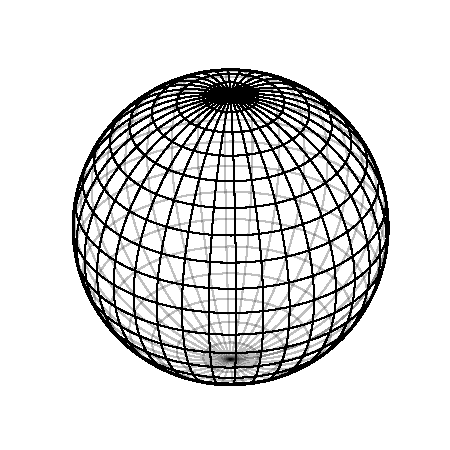
\includegraphics[width = 4in]{images/sphere.pdf}
	\end{center}
	\vfill
	\begin{center}
		{
			\Large
			\textsc{Sic Mundus Creatus Est}
		}
	\end{center}
\newpage
	\thispagestyle{empty}
	\begin{center}
		{
			\Large
			\textit{Ad Astra per Aspera}\\[2.5in]
			\textit{Hic sum, hic maneo}
			\vfill
			\textit{\textbf{Mors vincit Omnia}}
		}
	\end{center}
